% !TEX root = ../thesis-example.tex
%
\chapter{Geste instumental}
\label{ch:transparency}

\cleanchapterquote{La percussion de ce pseudo-gong est illlusoire : rien ne tape sur rien dans l’ordinateur. Schumann qualifiait le legato au piano de “trompe-l’oreille” : la musique est aussi un art du mirage, de l’illusion.}{Jean-Claude Risset}{Discours invité aux JIM 2010 \cite{risset_propos_2010}}


Les DMI introduisent un découplage énergétique, une dislocation du controle (\textit{control dislocation} \cite{miranda_new_2006}), rompant avec plus de 40.000 ans de tradition musicale \cite{conard_new_2009}.

\section{Introduction}
%-------------------------------------------
\subsection{Tout ce qui bouge n'est pas geste}

Dans le domaine de la recherche musicale, les mouvements du corps sont associés à la notion de \textit{geste musical}, c'est à dire à un concept associant à la fois le \textit{mouvement} du corps et \textit{l'intention} et/ou \textit{la signification} de ce mouvement. 

Cela n'est pas nécessairement et systématiquement le cas et les mouvements de l'instrumentiste peuvent être envisagés et décrits avec d'autres perspectives que celle de leur potentielle intention. \todo{ref ou footnote ici vers des études en ce sens} La notion de \textit{geste musical} semble en effet implicitement suggérer un rapport hiérarchique entre le musicien et son instrument, dans lequel les gestes ne serait produits qu'intentionnellement, à l'initiative du musicien.\todo{mal dit}. Les instruments de musique, et en particulier les DMIs, sont envisagés plus récemment comme \textit{agents} qui opèrent dans un système de relations multi-directionnelles\todo{ref}, que Berliner décrit métaphoriquement par une \textit{conversation} dans \cite{berliner_thinking_2009}. \todo{attention,il parle de la relation musicien/public} L'instrument vibre et produit parfois du son sans qu'il soit explicitement déclenché ou controlé. Les mouvements du corps du musicien en témoignent et au dela des effets spectaculaires des DJs qui touchent aux potentiomètres de leurs interfaces comme s'ils étaient brûlants \footnote{\url{https://www.youtube.com/watch?v=Nh9C7nQHmII}}, le corps est parcouru de mouvements qui ne sont pas uniquement des \textit{actions} mais des \textit{réactions} à ce qui est produit par l'instrument. 

Si l'on considère la relation geste/instrument/musique comme un réseau multi-directionnel, le geste peut-être provoqué par la musique, via l'instrument lui même. Deux exemples caricaturaux viennent illuster cette possibilité : la performance \iquote{eletric stimulus to face — test} de l'artiste Daito Manabe\footnote{\url{http://www.daito.ws/work/electricstimulustoface_test.html}} ou dans le terrifiant système de motorisation des doigts pour apprendre un instrument proposé par \cite{zhang_adaptive_2019}.

%-------------------------------------------
\subsection{Découplage énergétique}

Les \glspl{DMI} présentent non seulement un découplage énergétique entre les gestes du musicien et le résultat sonore, mais également une partie computationnelle couplée à une mémoire qui permet une re-programmation complète de l'interaction, rendant leur fonctionnement cryptique. Cet aspect peut se révéler être un inconvénient, dans la mesure où il prive le public d’une lecture possible de la performance musicale. Cela peut cependant s’avérer être un avantage, dans la mesure où la performance musicale comporte une part scénographique dans laquelle l’illusion a toute sa place.

Je présenterai dans ce chapitre quelques aspects sur la relation entre le geste musical et les \glspl{DMI}, en présentant les théories proposées par un certain nombre d'auteurs, et en proposant de les compléter par la considération de la part subversive du geste musical, en m'appuyant notamment sur une performance audio-visuelle réalisée avec la plasticienne Gladys Brégeon. Cette performance implique différents types d’interfaces, et pour chacune de ces interfaces, des interactions diverses et hybrides qui joue en partie sur la lecture souhaitée ou fantasmée de ce qui s’opère sur scène.

%%%%%%%%%%%%%%%%%%%%%%%%%%%%%%%%%%
\section{Revue des théories sur le geste instrumental}

Auteurs : Cadoz, Godoy, Leman, Wanderley, Camurri 

Le geste peut être étudié sous différentes perspectives, selon que l'on s'intéresse à lui en tant que vecteur de communication, d'action opérante ou encore de métaphore décrivant un mouvement, selon que l'on adopte une approche purement phénoménologique ou plus structurelle et fonctionnelle. [cf. Cadoz, C. 1994. "Simuler pour connaître..." ?]

% Une classification souvent citée est celle de Delalande, qui dans son étude des techniques de jeu de Glenn Gould, proposait trois catégories de gestes chez l'interprète, allant graduellement du ``purement fonctionnel au purement symbolique'' \todo{vérifier cette citation}:

% \vspace{-1em}
% \begin{itemize}[noitemsep]
% \item \textbf{les gestes effecteurs}, nécessaires à la production du son: pincement de cordes, déplacement de l'archet, pression d'une touche, etc.;
% \item \textbf{les gestes accompagnateurs (ou ancilaires)}, associés aux gestes effecteurs, engageant tout le corps, sans être directement nécessaires à la production du son : mouvements d'épaule, respirations du pianiste, etc.
% \item \textbf{les gestes figuratifs}, perçus par l'auditeurs sans être clairement reliés à des mouvements du corps : articulation mélodique, etc.
% \end{itemize}


Quatre catégories de gestes ont été distinguées dans \cite{jensenius_musical_2010} à partir des différentes contributions de Gibet \cite{gibet_codage_1987}, Cadoz \cite{cadoz_gesture_2000}, Delalande \cite{delalande_geste_1988}, Godøy \cite{godoy_exploring_2006}, Wanderley et Depalle\cite{wanderley_gestural_2004}:

\vspace{-1em}
\begin{itemize}[noitemsep]
\item \textbf{les gestes de production du son}, aussi appelés \textit{gestes instrumentaux} chez Cadoz [todo ref]  et \textit{gestes effecteurs} chez Delalande, nécessaires à la production du son: pincement de cordes, déplacement de l'archet, pression d'une touche, etc. Ils ont été sous-divisés par Cadoz \cite{cadoz_instrumental_1988} entre :
	\vspace{-1em}
	\begin{itemize}[noitemsep]
		\item \textbf{gestes d'excitation} qui fournissent l'énergie qui sera au présente dans le son \textit{in fine}. Ils peuvent être de nature \textit{continue}, quand le son et le geste co-existent (e.g. frottement de l'archet, souffle dans un instrument à vent), ou de nature \textit{instantanée}, si le son commence quand le geste finit (e.g. percussion, pincement de corde);
		\item \textbf{gestes de modification} venant modifier les propriétés de l'instrument. Ici, Cadoz distingue les modifications paramétriques, telles que le vibrato, et les modification structurelles, telles que l'insertion d'un accessoire (e.g. sourdine d'une trompette) ;
		\item \textbf{gestes de sélection}, consistant à choisir parmi plusieurs éléments similaires d'un instrument (e.g. quelle touche de piano).
	\end{itemize}
\item \textbf{les gestes de communication}, aussi appelés \textit{gestes sémiotiques} dans \cite{cadoz_gesture_2000} permettant une communication entre musiciens ou avec le public;
\item \textbf{les gestes facilitant le son}, aussi appelés \textit{gestes accompagnateurs} chez Delalande \cite{delalande_geste_1988} ou \textit{gestes ancillaires} par Wanderley et Depalle \cite{wanderley_gestural_2004} venant soutenir les gestes de production du son;
\item \textbf{les gestes accompagnant le son}, ne sont pas impliqués dans la production du son, mais suivent la musique. En particulier, Godøy distingue deux sous-catégories :
	\vspace{-1em}
	\begin{itemize}[noitemsep]
		\item \textbf{sound-tracing}, i.e. following the contour of sonic elements \cite{godoy_exploring_2006}
		\item \textbf{les gestes d'imitation} qui consistent à mimer ou imiter des gestes de production du son, comme il peut être observer dans les performances de \textit{air guitar}\footnote{Le \textit{air guitar} est une activité qui consiste à mimer le geste d’un guitariste, typiqument de guitare électrique dans un groupe de rock ou de métal, sans avoir l’instrument en main, dans une sorte de playback instrumental.} \cite{godoy_playing_2005}
	\end{itemize}
\end{itemize}


\noindent Wanderley ajoute à cette classification une distinction entre :
\vspace{-1em}
\begin{itemize}[noitemsep]
\item \textbf{Gestes sans contact physique} avec l'instrument : libre, sémiotique ou gestes nus;
\item \textbf{Gestures avec contact physique} : ergotique, haptique, gestes instrumentaux.
\end{itemize}


Notons que dans leur classification, Cadoz et Wanderley définissent le geste instrumental comme un geste \iquote{appliqué à un objet matériel et en interaction physique avec lui}, ajoutant que \iquote{les gestes nus (empty-handed gestures) ne sont pas des gestes instrumentaux pour la raison qu'il ne possède qu'une fonction sémiotique}.

On perçoit évidemment les limites de cette notion de contact physique, quand il s'agit d'instruments comme le theremin, ou quand des capteurs sans contacts tels que les capteurs de distance par ultra-son ou infra-rouge, les caméras vidéo, les kinect\footnote{interface conçue par Microsoft, qui s'apparente à une caméra fournissant, en plus d'une image vidéo classique, une carte de profondeur de l'image captée.}, leap-motion\footnote{interface conçue par Microsoft, qui s'apparente à une caméra fournissant, en plus d'une image vidéo classique, une carte de profondeur de l'image captée.} et autres radars... Le \textit{geste nu} s'apparente dans ce cas à un geste ergotique.

Au moment où il écrit cela, Wanderley considère que le nombre d'instruments sans contact physique est très réduit, ne citant que le Theremin comme exemple. Par ailleurs, l'IRCAM est marqué par une tradition musicale historiquement orientée vers la pratique instrumentale classique d'instrument acoustique, la partie \textit{electronique} des œuvres n'étant jamais vraiment considéré comme une partie instrumentale, et d'ailleurs, jamais \textit{jouée} par un musicien, mais délenchée par un \textit{\gls{RIM}}.

Depuis, le nombre de capteurs permettant une interaction sans contact physique n'a cessé d'augmenter et de se démocratiser : caméras vidéos, caméras 3D (e.g. kinect, leap motion), capteurs de distance à infra-rouge ou ultra-sons, capteurs photosensibles, gyroscopes et accéléromètres... Le nombre d'instrument présentant des gestes sans qu'il y ait de contact physique avec un objet n'a donc cessé d'augmenter.


Mulder \cite{mulder_mulder_2000} propose pour sa part une classification des gestes selon les caractéristiques physiques de l'objet manipulé
\vspace{-1em}
\begin{itemize}[noitemsep]
\item \textbf{Type d'objet} solide, liquide, fluide, gaz
\item \textbf{Changement opéré} : position, orientation, forme
\item \textbf{Numbre de mains impliquées}
\item \textbf{Niveau d'indirection} : manipulation directe ou à l'aide d'un autre objet ou outil
\end{itemize}


Delalande suggests that accompanist gestures should not be analyzed strictly from a motor control point of view — he considers that its function is as related to imagination as to the effective production of the sound. (in \cite{cadoz_gesture_2000})

Le problème de toute catégorisation est qu'elle peine à rendre compte des chevauchements et intersection entre ses catégories. Nommément, les gestes subversifs peuvent être de nature excitatoire tout en jouant sur le \textit{pré-geste} (sound-facilitating) pour lui faire dire le contraire.

D'autres descriptions du geste telles que celles employées dans l'apprentissage du Guqin

D'un certain point de vue, on pourrait dire que cela n'a pas de sens de vouoir jouer d'un DMI de manière \textit{transparente} dans la mesure où les gestes sont subvertis à la source même de l'interaction. C'est en quelque sort un mésusage de l'informatique qui consiste à l'utiliser comme si les DMI étaient des synthés analogiques (dans lesquels une certaine continuité énergétique subsiste entre les capteurs et le son).


%-------------------------------------------
\subsection{Le geste comme action}

\iquote{Nous appelons ici gestes de l’instrumentiste les actions physiques effectuées par le musicien en situation de jeu instrumentale.} \cite{wanderley_controle_1999}



Théorie de Cadoz: le canal

\vspace{-1em}
\begin{itemize}[noitemsep]
\item readable gesture to sound relations
\item confusing gesture to sound relations
\end{itemize}


Dans le domaine des \glspl{HCI} 

Pendant longtemps (TODO : combien?), les instrumentistes utilisant des \glspl{DMI} ont été cachés derrière des machines, à la position souvent occupé par l'ingénieur du son, ne laissant rien voir ou si peu de ce qu'ils faisaient vraiment. Pire, ils se trouvaient suspectés, quand ils étaient sur scène, 


Expliquer en quoi le découplage énergétique, qui a amené à "un sens de la discontinuité avec la tradition, aliénation et manque de compréhension par le public en ce qui concerne ce que l'instrumentiste ou l'instrument fait en réalité". (T Magnusson, in \cite{magnusson_sonic_2019} pp. 61) a amené à une contre-réaction faisant passer la lisibilité de la relation geste/son comme un critère pertinent de design instrumental.

%-------------------------------------------
\subsection{Le geste perçu}


%%%%%%%%%%%%%%%%%%%%%%%%%%%%%%%%%%
\section{Les limites d'une analyse des DMIs en terme de HCI}
\label{sec:transparency:limitesHCI}

Plusieurs articles des NIME analyse les DMI comme \gls{HCI} : 
Louange de la transparence : \cite{fels_mapping_2002}

Certains auteurs ont critiqué cette approche \cite{fyans_where_2009} en remarquant que l'idée selon laquelle une connaissance et une compréhension préalable de l'instrument et de l'idiome était nécessaire pour évaluer une performance musicale, ne pouvait être généralisée aux DMI, à cause de l'émergence rapide de technologies, d'instruments et de pratiques de performance dans ce domaine. 

Cependant, cette critique reste ancrée sur une approche qui considère que le spectateur évalue le \textit{succès} d'une performance selon sa compréhension des intentions de l'instrumentiste.



Le jeu musical joue en partie sur l’attente de l’audience (récompensée ou non) sur la base de règles d'harmonies, d’idiomes (e.g. cadences, résolutions, cycles rythmiques), de citations (e.g. via le sampling), etc..
Affordance des instruments ne peut être réduite aux objectifs d’affordance des HCI.


Kurtag Jr. Hangsimotato (video)
Jean Haury Meta-Piano
Applebaum Aphasia

gestes incongruent (Musical gestures, Godoy, p.48)


%-------------------------------------------
\subsection{Les musiciens ne sont \emph{pas} des utilisateurs d'instruments}
%-------------------------------------------
\subsection{La scène et le laboratoire}

Les instruments ne sont pas des interfaces utilisateurs.

Passé d'un rapport à la musique enregistrée du disque qui cherche une fidélité par rapport à l'enregistrement à la performance qui cherche à être fidèle au disque. \cite{??} 
Large développement d'outils pour la gestion "offline" de la musique (déplacement, copié/collé,etc) et de l'ergonomie de ces outils.
Hybridation des instruments entre du controle instrumental direct ("traditionnel") et des techniques issues de la production musicale offline.


accorde à la musique le droit de \iquote{tromper l'oreille} (et la vue).


%%%%%%%%%%%%%%%%%%%%%%%%%%%%%%%%%%
\section{Espace du geste musical}
La musique a longtemps été considéré comme étant faite d'un sous-ensemble de sons, les sons harmonieux, voire harmonique, avant qu'au XXème siècle, les bruits n'y fassent leur place avec les avant-gardes, futuristes. 

John Cage in \cite{cage_silence:_1961}
\begin{quotation}
\noindent If this word, music, is sacred and reserved for eighteenth- and nineteenth-century instruments, we can substitute a more meaningful term: organization of sound.\\
\end{quotation}


La musique n'est donc pas faite que de sons, au sens acoustique du terme, mais également (avant tout?) de la perception des sons, qui implique des processus de cognition, des références socio-culturelles, et une sensibilité, une mémoire propre à chacun. 
Ainsi, l'espace de la musique ne se présente non pas comme un sous-ensemble de l'espace des sons, mais probablement comme un sur-espace comprenant à la fois les sons acoustiques mais également tous les liens qu'ils tissent avec notre mémoire.

L'art musical consiste ainsi à faire entendre des aspects de la musique qui ne sont pas nécessairement présents dans le son, à faire surgir des espaces qui ne peuvent se déployer que dans notre imaginaire, en faisant écho à la trace latente que les sons et la musique ont déjà imprimée en nous.


\begin{quotation}
\noindent Le musical dépasse le sonore en cela qu’il est connecté à une expérience cognitive qui implique la perception et la mémoire.\\
Le sonore dépasse le musical en cela que tout ce qui est sonore ne fait pas nécessairement musique (sauf chez Cage).
\end{quotation}

Là où la présence du musicien sur scène remplissait une nécessité acoustique pour l’écoute, la musique sur support, ou produite par des machines, déplace ce besoin au profit d’une autre fonction, à la fois de compréhension des gestes du musicien (mais est-ce là un jeu de dupes?) et d’un spectacle de l’ordre du funambulisme; le musicien prend des risques [celui de se tromper dans le cas de l’interprétation d’une partition] et la mise en question du corps, réagir au contexte (lieu et au public, ainsi qu’aux éventuels autre musiciens) d’une manière vivante.

L’écoute nous plonge dans des flux sonores, et notre tendance à projeter des causes à ces sons (cf. gestalt) nous emmène sur les lieux — toujours en partie étrangers — de la production de ces flux. sitar indien, crissement de pneu, explosion, acoustique sous-marine ou ambiance de salle de café.
Le musicien crée des passerelles et des agencements entre ces zones liminales.

Si les gestes \textit{subversifs} peuvent être assimilés à des gestes accompagnateurs, la plupart des articles de la littérature semble ignorer cette part de subversion au profit de la lisibilité du geste et sa corrélation avec le son \cite{godoy_exploring_2006}.
Cependant, la corrélation n'est pas nécessairement recherchée en tant que telle et si, comme le rappelle Risset, \iquote{la musique est aussi un art du mirage, de l’illusion} \cite{risset_propos_2010}, les œuvres sont nombreuses qui cherchent à dépasser le lien d'apparente causalité entre le geste et le son. 
Il serait alors plus juste d'utiliser le terme de \textit{geste accompagnant la musique}, si toutefois on 

%---- Figure : Einarsson sculpture ---------
\begin{figure}[htb]
	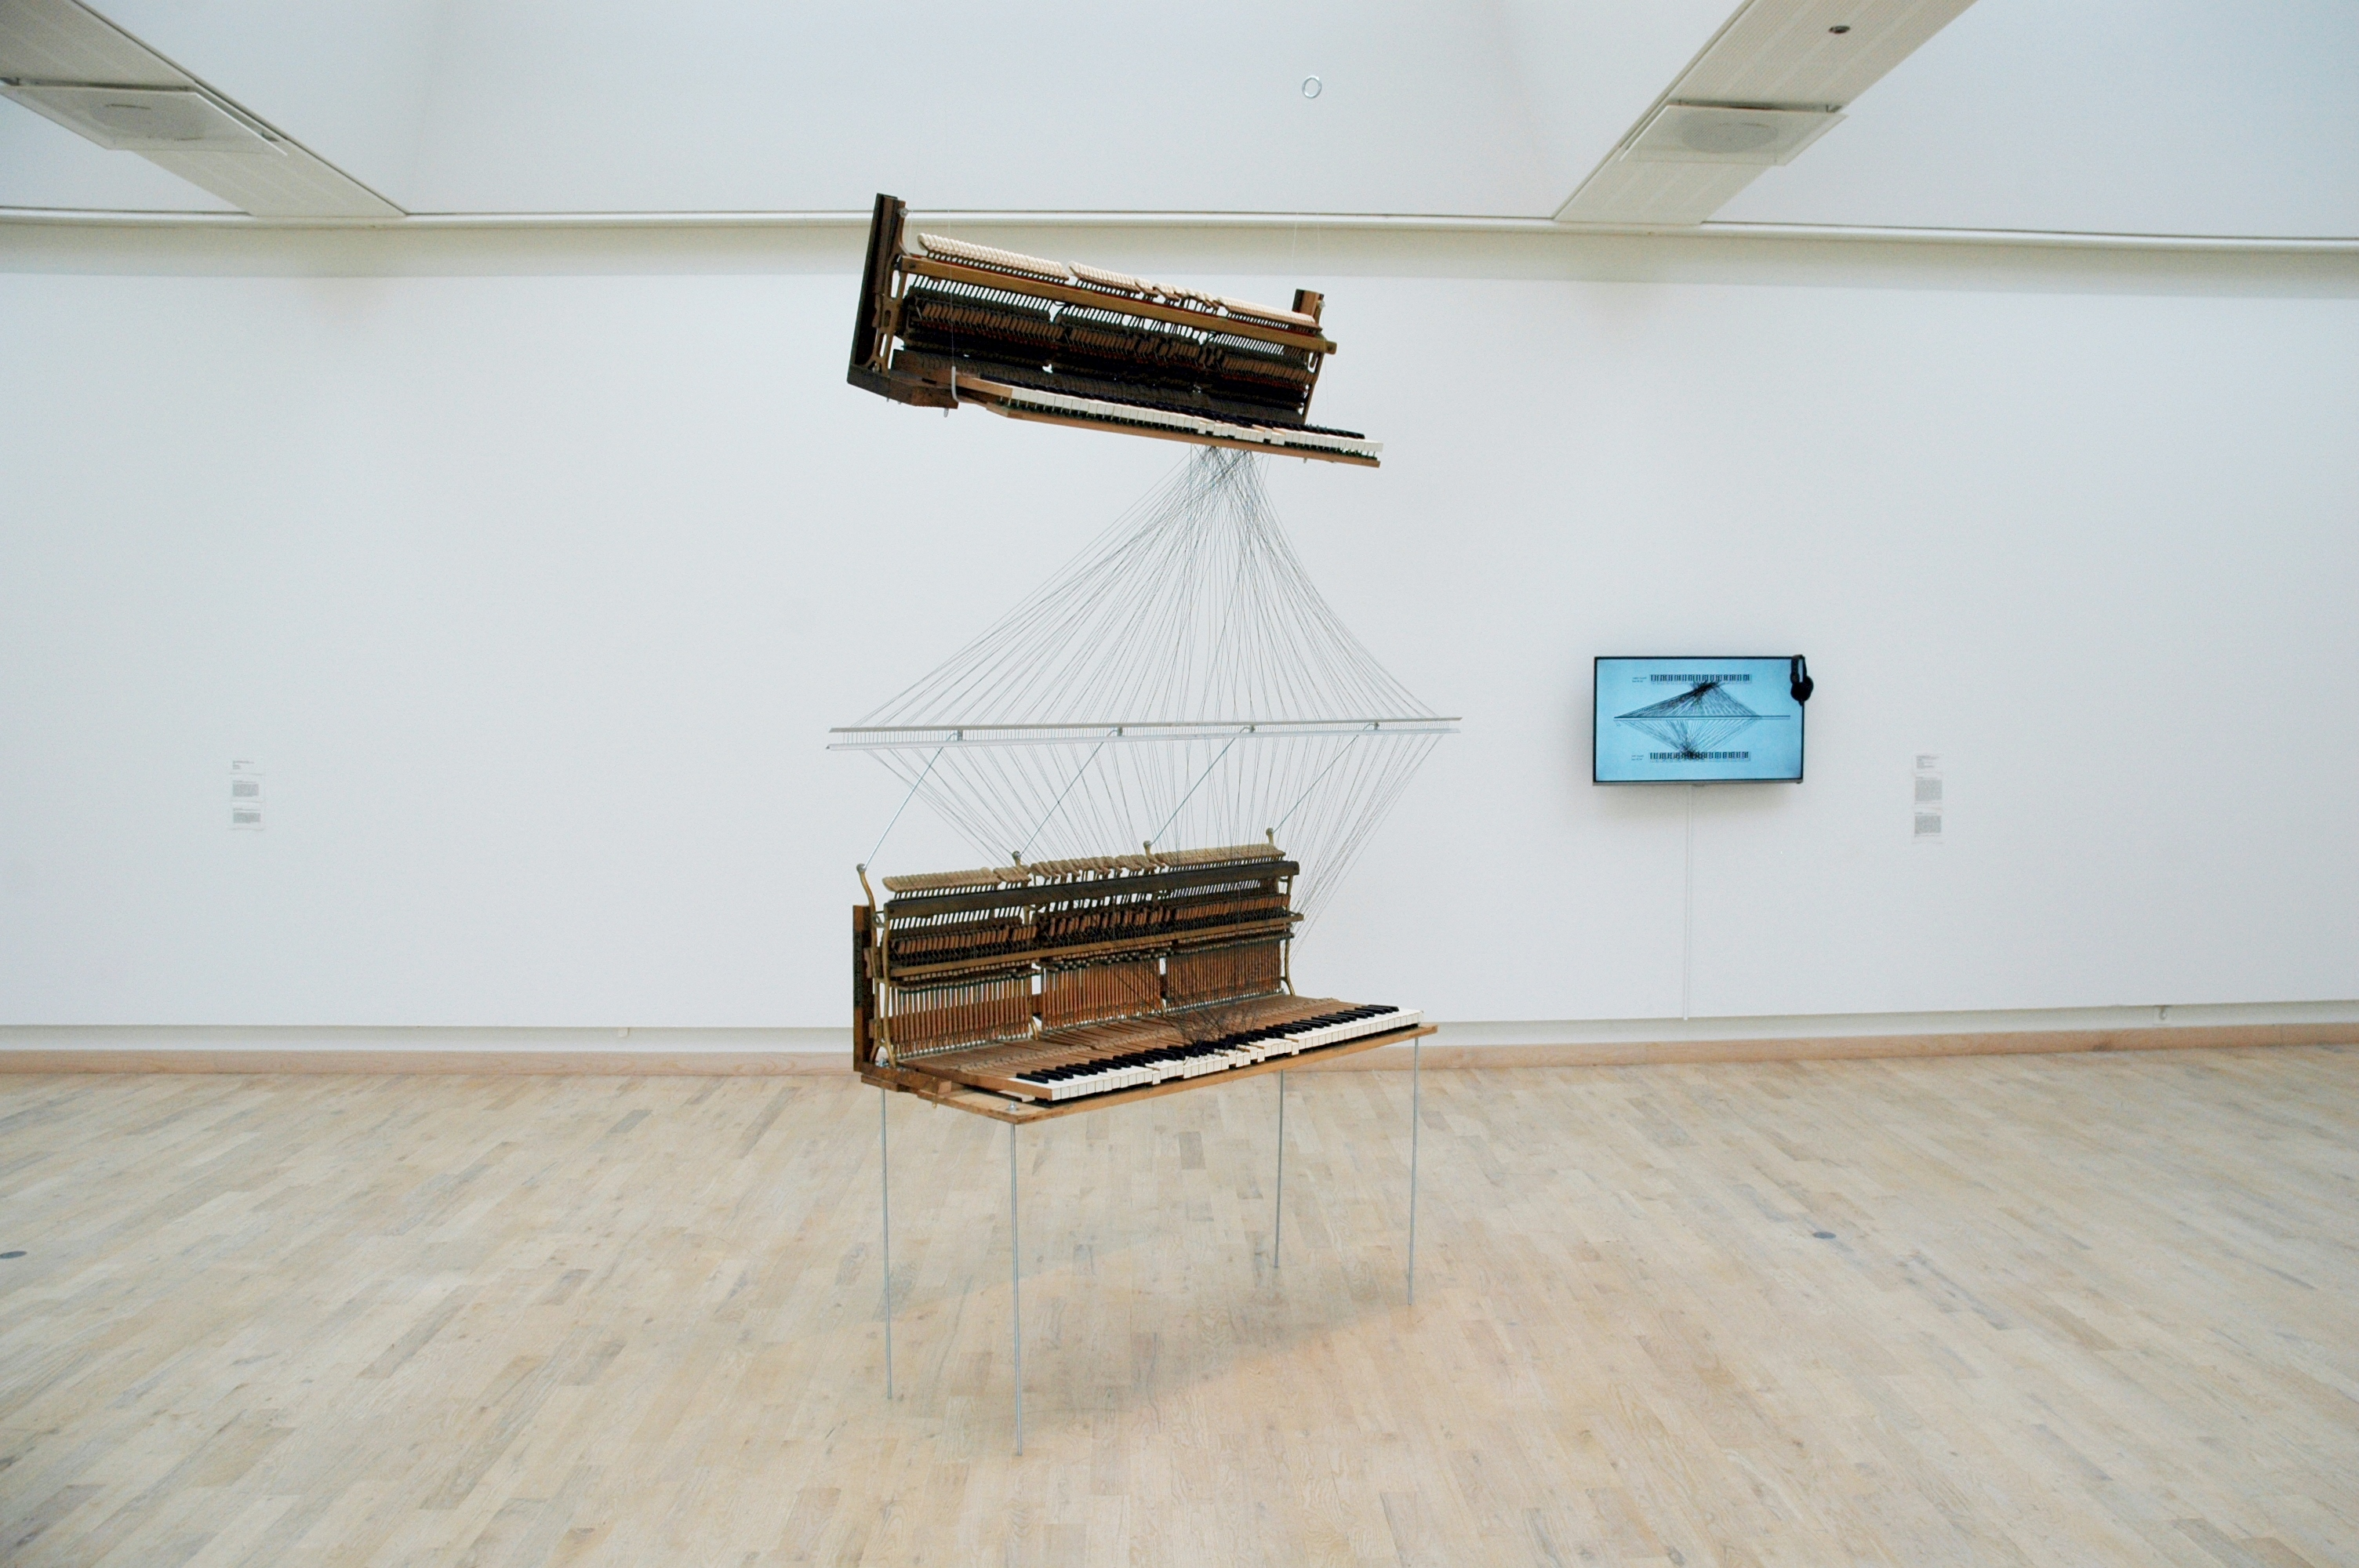
\includegraphics[width=\textwidth]{gfx/Einarson-SchumannSculpture}
	\caption{Einar Torfi Einarsson - Schumann-Sculpture (remnants + deracination)}
	\label{fig:gesture:einarsson}
\end{figure}


\iquote{Every music performance is a dramatic presentation for listeners and improvisers alike. In a sense, both groups play interactive roles as actors from their respective platforms. Just as the design of the hall, the stage and the lighting frames the band's activity for the audience's observation, it also frames the audience's activity for the band to observe. Performers and listeners form a communication loop in which the ction of each continuously affect the other.} Paul F. Berliner in \cite{berliner_thinking_2009}

%%%%%%%%%%%%%%%%%%%%%%%%%%%%%%%%%%
\section{Subversion sonore, subversion gestuelle}

La subversion peut intervenir à différents niveaux. Au niveau de la composition, l'écriture musicale permet des modulations qui déjouent les attentes de l'auditeur. (e.g. Pink Floyd, breathe transition). Elle peut également se situer au niveau du jeu, en usant de procédés comme des gestes qui contredisent ce qu'on entend et vont l'amplifier. Gyorgy Kurtag Jr. geste violent pour jouer une nuance pianissimo.

Exemples comparés de Applebaum Aphasia et Vincent Carinola/Jean Geoffroy "Rhizome".
BBC Classic Album: "Pink Floyd - The Dark Side of the Moon"

Dissonance cognitive.

Synchrèse de Michel Chion.

Parler du playback, du air-guitar, de la synchrèse.

Bien que ces catégorisations du gestes décrivent adéquatement différents aspects du geste instrumental sur des instruments acoustiques, il semble que le geste musical intègre une aspect subversif souvent négligé.

En particulier, dans le cas des \gls{DMI}, la relation entre le geste et le son est totalement sujette au design de ce que l'on nomme communément le \gls{mapping} et la part de subversion devient partie intégrante du design de ce mapping. 

Richard Leppert dans \cite{leppert_sight_1993} souligne à quel point la nature intangible du son et de la musique est polarisée par l'expérience visuelle :
\begin{quotation}
Precisely because musical sound is abstract, intangible, and ethereal [...] the visual experience of its production is crucial to both musicians and audience alike for locating and communicating the place of music and musical sound within society and culture. [...] Music, despite its phenomenological sonoric ethereality, is an embodied practice, like dance and theater." 
\end{quotation}

Il semble dès lors que l'on peut envisager d'autres types de relation entre le geste et le son, afin de tenter de décrire les différents rapports qu'ils entretiennent selon les situations.

Risset fait remarquer l'importance de l'histoire du son d'origine mécanique dans la perception des sons \cite[risset_son_1992]: 

\begin{quotation}
The limitations of digital acoustics depend upon the differential capacities of perception rather than upon the constraints of mechanics. Yet our auditory perception is geared to a world of mechanically-produced sounds, and mechanics should not be given a cavalier dismissal, as the work of Gibson and Cadoz has suggested : the specifics of mechanical vibrations shed light on the the perceptual organization in the hearing process.
\end{quotation}

\begin{quotation}
II semble à première  vue  que I'acoustique  numérique puisse  s'affranchir  de la mécanique. Cependant notre ouïe  a  évolué dans un  environnements d'objets vibrants: aussi la prise en considération  des  contraintes et des  particularités  des  vibrations  mécanique s  est-elle importante  pour  comprendre  les  idiosyncrasies de la perception  auditive et pour  en  tirer parti.
\end{quotation}


\textbf{Proposition}
\vspace{-1em}
\begin{itemize}[noitemsep]
\item readable gesture to sound relations
\item confusing gesture to sound relations
\end{itemize}

\vspace{-1em}
\begin{itemize}[noitemsep]
\item Gestes emphatique = en phase avec le mouvement interne du son
\item Geste apophatiques = en opposition de phase avec le son
\item Geste unrelated
\end{itemize}

%-------------------------------------------
\subsection{Continuités artificielles}

\vspace{-1em}
\begin{itemize}[noitemsep]
\item Contrepoint : relier la mélodie à l'harmonie 
\item Bach et le tempérament = relier les différents modes, via la modulation.
\item les doigtés alternatifs, sur le plan gestuel, permettent de sacrifier la justesse de la note, pour établir une continuité gestuelle fluide
\item La musique sérielle : relier la gamme tempérée au spectre en ordonnant 
\item Stravinsky, Russolo : relier l’harmonie et le bruit 
\item jouer un pattern connu ("qu'on a dans les doigts") tout en substituant les notes permet de jouer de manière fluide une mélodie inhabituelle. => numérique
\item Cage, Murray Schaeffer : relier le déterminisme et le hasard, la musique et l’environnement 
\end{itemize}

=> voir Théories de la composition musicale au XXe siècle 
Conjointement à ces explorations compositionnelles se sont développées des techniques et des technologies permettant d’appréhender ces nouveaux espaces. Que cela soit des procédés d’écriture ou des instruments reflétant ces méthodes et modèles.



%-------------------------------------------
\subsection{Dans les instruments traditionnels}

%-------------------------------------------
\subsection{Dans les instruments numériques}


Les DMI ont souvent été analysés en tant qu'interface homme-machine, et les conférence académique qui leur sont consacrés reflètent une culture dans lequel l'interaction s'exprime via un cahier des charges préalablement identifié: une interface homme-machine est utilisée dans le cas d'une tâche précise et sa qualité (ergonomie, précision, etc.) peut être mesurée de manière quantifiée.
Dans le cas des instruments de musique cependant, cette tâche est plus complexe, car les enjeux de la création musicale dépassent par essence tout objectif identifié et mesurable au préalable. Par ailleurs, les DMI sont destinés plusieurs types "d'utilisateurs" ayant un rôle différent : le musicien qui joue de l'instrument, mais également le public, qui bien qu'il ne joue pas de l'instrument est amené à en observer la performance.

Low entry fee, high ceiling.

La performance musicale est un "jeu" qui comporte une part de duplicité. Le public d'un concert est toujours le sujet d'une illusion. 

Un des biais de la littérature sur l’affordance des instruments de musique numérique est qu’elle s’inspire souvent des objectifs de l’affordance des HCI en général, avec l’idée que l’instrument doit être compréhensible pour les “autres” utilisateurs potentiels que l’auteur de l’instrument. Pourtant, nombre d’instruments présentés dans la communauté NIME ne sont joués que par leurs auteurs (cf. [1], [2], [3]) et si le fait de vouloir transmettre son instrument aux autres est louable, il n’est pas gage de qualité en ce qui concerne la création qui sera faite avec cet instrument.     


L'art musical procède en partie de la magie et de l'illusion perceptive. Le musicien nous fait entendre des continuités (e.g. une mélodie) là où l'acoustique fait apparaitre une série discrète (e.g. des notes de piano), ou inversement des fissions (e.g. deux voix indépendantes) là où est jouée une série temporelle de notes sur un même instrument. (=> plutôt que des exemple entre parenthèse, mettre une figure illustrant fission e.g. Bach's Violin Partita No. 3, BWV 1006.)

Cette question du jeu entre le continu et le discret dépasse le seul cadre de la musique mais semble trouver dans cet art de nombreuses espaces d'expression.

Les théories de la perception, en particulier du Gestalt, viennent en partie expliquer les mécanismes qui pousse notre perception à créer des continuités où il n'en existe pas physiquement et inversement à catégoriser des événements selon certaines distances perceptives qui ne sont pas nécessairement en lien avec l'unité de source de production du son.

Si donc on analyse le geste musical, il faut nécessairement prendre en compte sa dimension subversive en ce qu'elle se traduit, particulièrement dans le cas des DMIs et des productions musicales impliquant l'électronique en général, dans le design des instruments et outils qui servent à la créer.

\cite{bin_show_2018}

Carte et guide , frettage adaptatif (cite pitch)

\section{Morpho-dynamisme dans les DMI}

Mettre capture d'image du MID qui passe d'une structure rotative à un Verlet.

Comment la continuité s'établit ?

\clearpage

\section{Co-performance}
Ainsi, la nature dynamique et générative des DMIs déplace l'agentivité de l'interaction instrumentale, qui ne saurait être réduite à une relation unidirectionnelle, où le retour haptique et/ou vibratoire n'aurait qu'une dimension épistémique et informative pour le musicien.
L'instrument peut se retrouver en position de mener le jeu et imposer sa cadence à l'instrumentiste. La performance musicale avec un DMI est donc une co-performance où la distribution du contrôle de la synthèse et de la gestuelle qui la provoque, ou en découle, peut se distribuer de manier polymorphe. Une partie de la dynamique de jeu peut être prise en charge par la machine et une autre partie par l'instrumentiste dans une relation qui peut parfois s'approcher d'un duo.

 La performance musicale avec un DMI est donc une co-performance où le contrôle de la synthèse est distribué entre la machine et le musicien. 
 Les gestes du musiciens ne sont ainsi par nécessairement des gestes de contrôle (puisqu'il peuvent être "libérés" de cette fonction là) mais peuvent \textit{découler} de la synthèse opérée par la machine. Les gestes du musicien peuvent alors entretenir des relation de nature différentes :

\vspace{-1em}
\begin{itemize}[noitemsep]
\item une relation d'accompagnement, cohérente ou dissonante;
\item une relation de réaction épidermique;
\item une relation neutre.
\end{itemize}
 


 
\section{Conclusion}
\label{sec:transparency:conclusion}
=> Comment ces aspects influencent le design de l’instrument ?

\section*{Conclusion}
Notion de vivadi

